\subsection{Hubble Constant from
\texorpdfstring{$\chi$}{χ} Dynamics}
\label{subsec:hubble-constant-from-chi-dynamics}

The Hubble parameter arises as an effective quantity:
\begin{equation}
  H(t) = \frac{\dot{\chi}}{\chi}.
\end{equation}
Assuming $\dot{\chi}_{\mathrm{eff}} \simeq c$, the present-day value is
$H_0 \simeq c/\chi(t_0)$.
Early- and late-universe probes sample~$\chi$ at different relaxation
stages, naturally leading to systematically different inferred values
of~$H_0$ without invoking additional cosmological components.

\paragraph{Resolution of the Hubble tension.}
The effective $H(z)$ acquires a mild redshift dependence departing from
$\Lambda$CDM at intermediate redshifts
($0.1 \lesssim z \lesssim 10$), testable through upcoming BAO and
supernova surveys.

\begin{figure}[t]
  \centering
  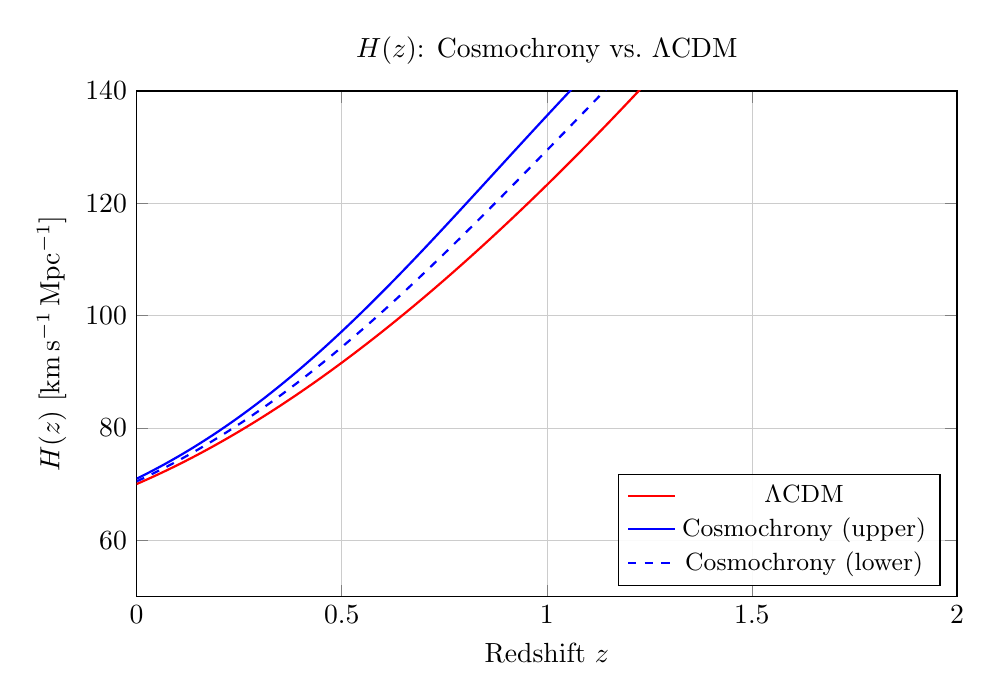
\begin{tikzpicture}
    \begin{axis}[
      width=12cm, height=8cm,
      title={$H(z)$: Cosmochrony vs.\ $\Lambda$CDM},
      xlabel={Redshift $z$},
      ylabel={$H(z)$ [km\,s$^{-1}$\,Mpc$^{-1}$]},
      xmin=0, xmax=2, ymin=50, ymax=140,
      xtick={0,0.5,1,1.5,2},
      legend style={
        at={(rel axis cs:0.98,0.02)},
        anchor=south east, draw=black,
        fill=white, fill opacity=0.9,
        text opacity=1, font=\small},
      grid=both,
      grid style={line width=.1pt, draw=gray!10},
      major grid style={line width=.2pt, draw=gray!40},
    ]
      \addplot[domain=0:2, samples=200,
        red, thick, mark=none]
        {70*sqrt(0.3*(1+x)^3 + 0.7)};
      \addlegendentry{$\Lambda$CDM}
      \addplot[domain=0:2, samples=200,
        blue, thick, mark=none]
        {70*sqrt(0.3*(1+x)^3+0.7)
          *(1+0.10*exp(-2*(x-1)^2))};
      \addlegendentry{Cosmochrony (upper)}
      \addplot[domain=0:2, samples=200,
        blue, thick, dashed, mark=none]
        {70*sqrt(0.3*(1+x)^3+0.7)
          *(1+0.05*exp(-2*(x-1)^2))};
      \addlegendentry{Cosmochrony (lower)}
    \end{axis}
  \end{tikzpicture}
  \caption{Schematic comparison of $H(z)$.
    Cosmochrony predicts a mild enhancement at intermediate
    redshifts due to relaxation inhomogeneities.}
  \label{fig:hubble-comparison}
\end{figure}
